\section{Prevalence of Suboptimality}
\todo{Sabah has modify token: rewrite according to the model}
\todo{path analysis}
As explained in Section~\ref{sec:datasets}, we looked
for query suboptimality among 500 randomly generated, quite simple queries,
for which the actual cardinality was known (the experiment scenario updated
the statistics before each plan was optimized). We observed that 266 of
these queries, or 53.2\%, were suboptimal.  This percentage comes with several
provisos. First, there were no foreign key constraints nor indexes, which in
some ways renders the optimizer's job harder.  Perhaps with
queries over data with more comprehensive schema available, the percentage
would be less. Second, for half of the suboptimal queries, the optimal plan
not chosen was within 30\% of the optimal plan (see
Figure~\ref{fig:time}). That said, that also means that there were a good
number of queries for which the selected plan was quite a bit off (with a
few running twice as long as the best plan for that query).

\begin{figure}[bth]\centering
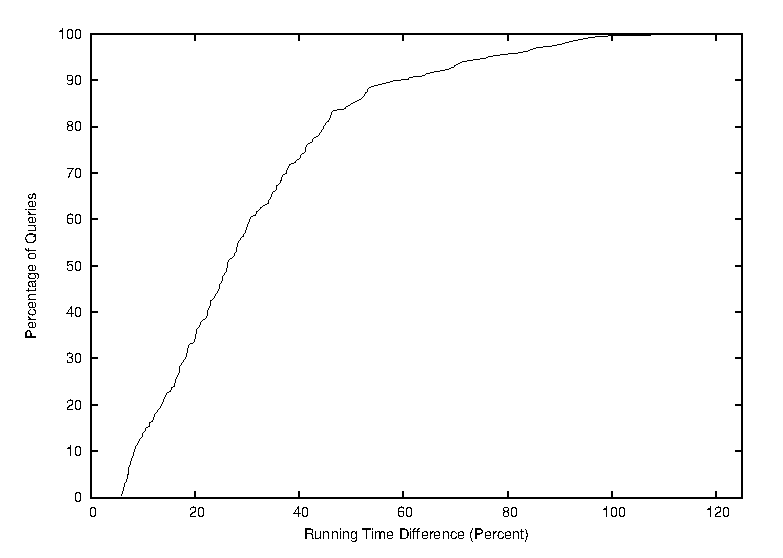
\includegraphics[width=0.50\textwidth]{figures/runtime_diff.eps}
\caption{Cumulative percentage of queries differing from the optimal plan by
  the indicated percentage of time\label{fig:time}}
\end{figure}

It is also interesting to look at the {\em width} of suboptimality: the
range of cardinality for which the optimizer {\em didn't} choose the optimal
plan. This width is defined to be the interval
of suboptimality starting from the cardinality immediately at the first
faster plan, extending across the actual cardinality of 1M tuples, to the
end of the cardinality of the last faster plan.

If the query optimizer is well behaved, one would might expect that the
optimal plan is relatively close, cardinality-wise, from the plan chosen by
the query optimizer, and this is indeed the case. Figure~\ref{fig:width} shows
the cumulative percentage of suboptimal queries exhibiting a width greater
than or equal to the width shown on the $x$-axis, expressed in cardinality
(number of tuples, in steps of 100K tuples), as specified by the {\tt
  searchGranularity} attribute in the {\tt variable\-TableSet} element of the
XML specification in Figure~\ref{fig:expspec}. The assumption of a
relatively close faster plan implies a concave cumulative distribution, as
was observed.

There is a big jump at 990,000, with this width accounting for about a third
of the queries. This occurs when there are two plans that are structurally
similar (as discussed later in Section~\ref{sec:ceps}) but have different
execution times, when measured at cardinalities of 1M and
2M (that is, at the {\em actual} and {\em maximum} cardinalities, for which
the experiment always obtains an execution time). By definition, this
particular circumstance translates to a width of $1\hbox{M} - 10\hbox{K} =
990\hbox{K}$.

\begin{figure}[bth]\centering
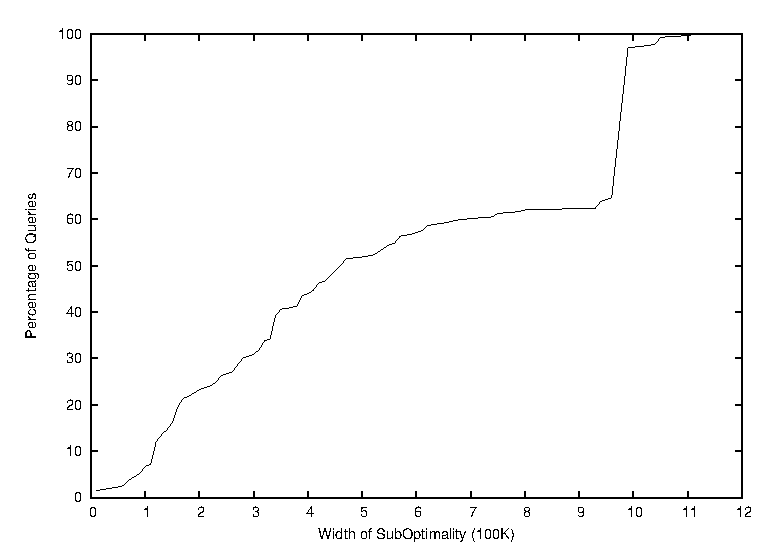
\includegraphics[width=0.50\textwidth]{figures/width_cumulative.eps}
\caption{Cumulative percentage of queries by
  the indicated width\label{fig:width}}
\end{figure}


\c2j{}{


\begin{table}[t]
\begin{center}
\begin{tabular}{c|c}
{\em DBMS} & {\em Percentage of Suboptimality}\\
\hline
{\bf A} & X\%\\
{\bf B} & X\%\\
{\bf C} & X\%\\
{\bf D} & X\%
\end{tabular}
\end{center}
\caption{Percentage of Suboptimality by DBMS\label{tab:dbmsprev}}
\end{table}

Second, suboptimality is highly variable, ranging from {\todo: X} to {\todo: Y}
queries (out of 100) for DBMS~{\todo: X}.

Third, even for very simple queries, suboptimality is quite prevalent.
Across all DBMSes, the prevalence is about {\todo: X}\%: {\todo: Y} of all
simple queries exhibit suboptimality. So it is likely that most extant
database applications include one or more queries that suboptimality.

\begin{table}
\begin{center}
\begin{tabular}{c|c|c}
{\em Number of} & {\em Number of} &{\em Percentage of}\\
{\em DBMS(es)} & {\em Suboptimal Queries} & {\em Suboptimality} \\
\hline
4 & X & X\% \\
3 & X & X\% \\
2 & X & X\% \\
1 & X & X\% \\
\end{tabular}
\end{center}
\caption{Prevalence of Suboptimality Across DBMS(es)\label{tab:supoptacross}}
\end{table}

Fourth, suboptimality is observed on different queries for different DBMSes.
Table~\ref{tab:supoptacross} 
summarizes the common suboptimal queries across multiple \hbox{DBMSes}.
We notice that {\todo: some phenomenon} 
all four \hbox{DBMSes}.
}

\section{Testing the Predictive Model}
\section{Sabah, change this also}
Our theory, that unanticipated interactions within the optimizer cause
suboptimality, coupled with the associated model in Figure~\ref{fig:model}, can be used
to derive specific predictions.  Simply put, we predict that as optimizer
complexity increases, so will suboptimality prevalence. However, as that is
a latent variable, not subject to direct control nor measurement,
we need to operationalize the independent variable of
optimizer complexity. Here we examine two such operationalizations of optimizer
complexity that we {\em could} control for, to render optimizer complexity
an independent variable.

\subsection{Impact on Query Parameters}
We first examine the relationship between
the prevalence of suboptimality and various aspects of the queries. For this
purpose, we considered the query parameters that are under our control: the
number of columns in the SELECT list, the number of correlation names in the
FROM list, and the number of self-joins in the WHERE clause. Our model
relates the query complexity to the number of plans. Of these independent
variables, only the number of correlation names in the FROM list will impact
the number of plans.

Our theory predicts that the higher the complexity of the optimization, that
is, the more correlation names in the FROM clause,
the higher the chance that the query will be suboptimal.

\begin{quote}
{\bf Hypothesis H1}: Suboptimality prevalence will correlate positively
with the number of correlation \hbox{tuple} variables used in the query.
\end{quote}

\begin{table}[t]
\begin{center}
\begin{tabular}{c|c|c|r}
{\em Number of} & {\em Number of} & {\em Number of} & \multicolumn{1}{|c}{\em Suboptimality}\\
{\em Corr Names}&{\em Queries}&{\em Suboptimal}&{\em Prevalence}\\
{\em in} FROM&&Queries&\\
\hline
1 & 113 & 5 & 4\%\\
2 & 136 & 57 & 42\%\\
3 & 117 & 91 & 78\%\\
4 & 134 & 113 & 84\%
\end{tabular}
\end{center}
\caption{Prevalence of Suboptimality by Number of Correlation Names in
FROM\label{tab:numcnfrm}}
\end{table}

As indicated in Table~\ref{tab:numcnfrm}, our experiment shows that the percentage of suboptimality grows
monotonically as the number of correlation names in the FROM clause
increases. \c2j{}{When looking at each individual experimental DBMS separately,
this trend is still present (see Figure~\ref{fig:numcnfrm}). (Note that the
number of columns were uniformly chosen to be 1 to 4, which implies a mean
of about 2.5 in the second column. For DBMS~{\bf C}, the number of columns
was fixed at 2, 4, 6, 8, and 10, for a mean of about 6.)} \c2j{A two-sample
  \hbox{t-test} assuming unequal variances shows that the mean
  number of correlation names for optimal
  queries, 1.8, as compared with that for suboptimal queries, 3.1, rejects
  the null hypothesis that they are drawn from the same distribution, with a
  {\em p-value} of $p<0.001$.}{The t-test results
in Table~\ref{tab:ttests}(c) reject the null hypothesis in all cases, 
as predicted by our theory. (We note that the query generation algorithm 
ensures that the number of predicates is the same as the number of 
correlation names in FROM clause. This might have played a role.)

\begin{figure}[t]
\begin{center}
\comment{\epsfig{file=figures/subopt_from/subopt_from.eps, width = 20pc}}
\end{center}
\caption{Prevalence of Suboptimality by the Number of Correlation Names in
FROM, by DBMS\label{fig:numcnfrm}}
\end{figure}

\begin{table}[t]
\begin{center}
\begin{tabular}{c|c|c|r}
{\em Number of} & {\em Number of} & {\em Number of} & \multicolumn{1}{|c}{\em Suboptimality}\\
{\em Corr Names}&{\em Queries}&{\em Suboptimality}&{\em Prevalence}\\
{\em in} FROM&&&\\
\hline
1 & 21 & 0 & 0\%\\
2 & 27 & 0 & 0\%\\
3 & 26 & 6 & 23\%\\
4 & 26 & 17 & 65\%
\end{tabular}

\vspace*{1em}

{\bf (b)} DBMS {\bf A} VaryStats Scenario

\vspace*{1em}

\begin{tabular}{c|c|c|r}
{\em Number of} & {\em Number of} & {\em Number of} & \multicolumn{1}{|c}{\em Suboptimality}\\
{\em Corr Names}&{\em Queries}&{\em Suboptimality}&{\em Prevalence}\\
{\em in} FROM&&&\\
\hline
1 & 21 & 0 & 0\%\\
2 & 27 & 5 & 19\%\\
3 & 26 & 7 & 27\%\\
4 & 26 & 3 & 12\%
\end{tabular}

\vspace*{1em}

{\bf (b)} DBMS {\bf A} Upper Scenario

\vspace*{1em}

\end{center}
\caption{Prevalence of Suboptimality by Number of Correlation Names in
FROM\label{tab:numcnfrm}}
\end{table}

\begin{table}[t]
\begin{center}
\begin{tabular}{c|c|c|c|l}
{\em DBMS}/ & {\em Mean} & {\em Mean} & {\em Statistic} &
{\em P value} \\
{\em Scenario}&{\em Optimality} & {\em Suboptimality} &\\
\hline
{\bf A} VaryStats&2.22&3.74&$p < 0.001$\\
{\bf A} Upper&2.52&2.87&$p< 0.001$\\
{\bf B}&X&X&X\\
{\bf C}&X&X&X&X\\
Overall&X&X&X&X\\
\end{tabular}
\end{center}
\caption{t-test Results for the Number of Correlation Names in the FROM Clause\label{tab:ttests2}}
\end{table}


\begin{table}
\begin{center}
\begin{tabular}{c|c|c|r}
{\em Number of} & {\em Number of} & {\em Number of} & \multicolumn{1}{|c}{\em Suboptimality}\\
{\em Columns}&{\em Queries}&{\em Suboptimality}&{\em Prevalence}\\
{\em in} Select&&&\\
\hline
1 & X & X & X\%\\
2 & X & X & X\%\\
3 & X & X & X\%\\
4 & X & X & X\%
\end{tabular}
\end{center}
\caption{Prevalence of Suboptimality by the Number of Columns in
SELECT\label{tab:numcnsel}}
\end{table}

The impact of the number of self-joins on the query optimization complexity, 
and thus, on the suboptimality prevalence as predicted by our theory,
is unclear. Hence, our theory is silent on the effect. {\todo: verification is
needed.}

As indicated by Table~\ref{tab:numselfjoin}, although as the number of
self-joins grows from zero to two, {\todo: complete with new observation}
%the percentage of flutters grows, it
%drops when number of self-join is three. In our 1000-queries data set,
%there are only six (=24/4, as there are four identical 1000-query sets) 
%queries with three self-joins, thus there isn't a large
%enough sample space to draw conclusions in this case. We do note that for
%all DBMSes the null hypothesis for number of self-joins is rejected. 
%It is unclear whether this is due to an increase in query optimization complexity, 
%or is due to a confounding increase in the number of correlation names (if so, 
%our theory would predict an increase in flutter), or is due to some other factor.

\begin{figure}
\begin{center}
\comment{\epsfig{file=figures/subopt_selfjoin/subopt_selfjoin.eps, width = 20pc}}
\end{center}
\caption{Prevalence of Suboptimality by Number of Self-Joins, by
DBMS\label{fig:numselfjoin}}
\end{figure}

\begin{table}
\begin{center}
\begin{tabular}{c|c|c|r}
{\em Number of} & {\em Number of} & {\em Number of} & \multicolumn{1}{|c}{\em Suboptimality}\\
{\em Self-Joins}&{\em Queries}&{\em Suboptimality}&{\em Prevalence}\\
\hline
0 & X & X & X\%\\
1 & X & X & X\%\\
2 & X & X & X\%\\
3 & X & X & X\%

\end{tabular}
\end{center}
\caption{Prevalence of Suboptimality by Number of
Self-Joins\label{tab:numselfjoin}}
\end{table}

As discussed in Section~\ref{sec:setup}, many of the queries included
self-joins, and about a third included two or more correlation names over the
independent variable table. Does varying the size of a self-joined table
induce more or less occurrences of suboptimality? Again, our theory is silent
on this. We performed a chi-squared test to see if the distribution of
suboptimality in the presence of a self-join on the varying
table was independent from the distribution of suboptimality in the presence
of a self-join not on the varying table. We found that the null hypothesis was 
rejected in this case ($\chi^2(1)=X,\,p<Y$). Interestingly, 
as shown by Table~\ref{tab:corSelfVar}, the prevalence of suboptimality
decreased when there was a self-join on the variable table.
{\todo: verification}

\begin{table}
\begin{center}
\begin{tabular}{c|c|c|c}
{\em Self-Join} & {\em Optimality} & {\em Suboptimality} & {\em Suboptimality Prevalence}\\
\hline
{\em Non-Variable} & X & X & X\% \\
{\em Variable} & X & X & X\%
	
\end{tabular}
\end{center}
\caption{Correlation Between Existence of Self-Joins on the Variable Table and Prevalence of Suboptimality\label{tab:corSelfVar}}
\end{table}
}

\c2j{}{
\subsection{Number of Operators}
One measure of optimizer complexity is the number of operators used by a
DBMS. The thinking here is that optimizers that have a lot of alternatives
at their disposal for common algebraic operators (scans and joins) will have
more inherent complexity in choosing among those operators.

\begin{quote}
{\bf Hypothesis H3}: Suboptimality prevalence will correlate positively
with the number of operators generated by the DBMS.
\end{quote}

We analyzed all the plans and accumulated the operators used by each DBMS;
the result is shown in Table~\ref{tab:ops}. Here the correlation is quite
striking. In fact, it appears that suboptimality percentage might be 
correlated with the square of number of operators, which makes some sense,
because optimizer interactions might be related to inter-operator
combinations.{\todo: verification}

\begin{table}
\begin{center}
\begin{tabular}{c|c|c|l}
{\em DBMS} & {\em Number of} &{\em Suboptimality} & {\em Operators}\\
& {\em Operators} && \\
\hline
{\bf C} & X & X\% &NestedLoop\\
{\bf A} & X & X\% &SeqScan,HashJoin\\
{\bf D} & X & X\% &SeqScan,HashJoin,\\
&&&Sort,MergeJoin\\
{\bf B} & X & X\% & SeqScan,\\
&&&Hash,HashJoin,\\
&&&Sort,MergeJoin,\\
&&&NestedLoop\\
\end{tabular}
\end{center}
\caption{Prevalence of Suboptimality by Number of Operators\label{tab:ops}}
\end{table}
}

\subsection{Effective Plan Space}\label{sec:ceps}
\c2j{One latent variable that is linked to optimizer complexity is the
  size of the plan space considered by the optimizer for each specific query.}{The number of operators a DBMS uses is a quite coarse independent variable
for optimizer complexity. Perhaps the size of the plan space considered by
the optimizer for each specific query is a better measure.} An optimizer that
can enumerate many plans (from a collection of many available operators) for
a query would expose that query to more complex interactions between
optimizer rules than a query for which the optimizer that enumerated just a
few plans, using a small set of operators.

While we did not have access to the number of enumerated plans (DBMSes do
not report such information), we do know how many unique plans were
generated for each query as we varied the estimated cardinality of one of
the tables. We consider two plans to be
different if they have different {\em structure}, that is, a different join
order, a different tree structure, or use a different physical operator
somewhere in the plan. We term the set of plans that were actually generated the {\em
  effective plan space}\c2j{ and}{; for Query~{\bf X} in
Figure~\ref{fig:subopt_instance}, that set is 
$\{$Plan 0, Plan 1, Plan 2, Plan 3, Plan 4$\}$.  We} term the size of this set
the {\em cardinality of the effective plan space}, or {\em CEPS}. Our
refined hypothesis predicts that queries that utilize more of the query
optimizer, that is, have a higher CEPS, will exhibit more suboptimality.
(We note here the pioneering work in the Picasso project,
which graphically depicted the plans chosen for
different cardinalities~\cite{harish07,reddy05},
thereby providing a visual representation of CEPS for a query.)

\begin{quote}
{\bf Hypothesis \c2j{H2}{H4}}: Suboptimality prevalence will correlate positively
with the cardinality of the effective plan space.
\end{quote}

\begin{table}[t]
\begin{center}
\begin{tabular}{c|c|c|r}
{\em CEPS} & {\em Number of} & {\em Number of} & \multicolumn{1}{|c}{\em Suboptimality}\\
&{\em Queries} & {\em Suboptimal} &  \multicolumn{1}{|c}{\em Prevalence}\\
&&{\em Queries} & \\
\hline
1 & 157 & 34 & 22\%\\
2 & 117 & 45 & 38\%\\
3 & 74 &58 & 78\%\\
4 & 73 & 62 & 85\%\\
5 & 50& 41 & 82\%\\
6 & 22& 20 & 91\%\\
7 & 5& 5 & 100\%\\
8 & 2& 1 & 50\%\\
\end{tabular}
\end{center}
\caption{Prevalence of Suboptimality by CEPS\label{tab:ceps}}
\end{table}

\c2j{}{\begin{table}[t]
\begin{center}
\begin{tabular}{c|c|c|c|r}
{\em DBMS} & {\em CEPS} & {\em Number of} & {\em Number of} & \multicolumn{1}{|c}{\em Suboptimality}\\
&&{\em Queries} & {\em Suboptimality} &  \multicolumn{1}{|c}{\em Prevalence}\\
\hline
{\bf A} & X & X & X & X\%\\
{\bf A} & X & X & X & X\%\\

{\bf B} & X & X & X & X\%\\
{\bf B} & X & X & X & X\%\\

{\bf C} & X & X & X & X\%\\
{\bf C} & X & X & X & X\%\\

{\bf D} & X & X & X & X\%\\
{\bf D} & X & X & X & X\%\\
\end{tabular}
\end{center}
\caption{Prevalence of Suboptimality by CEPS, per DBMS\label{tab:ceps}}
\end{table}

\begin{table}
\begin{center}
\begin{tabular}{c|c|c|c|r}
{\em Number of} &{\em CEPS} & {\em Number of} & {\em Number of} & \multicolumn{1}{|c}{\em Suboptmality}\\
{\em Tables}&&{\em Queries} & {\em Suboptmality} &  \multicolumn{1}{|c}{\em Prevalence}\\
\hline
2 & X &X & X & X\%\\
2 & X &X & X & X\%\\

4 & X &X & X & X\%\\
4 & X &X & X & X\%\\

6 & X &X & X & X\%\\
6 & X &X & X & X\%\\

8 & X &X & X & X\%\\
8 & X &X & X & X\%\\

10 & X &X & X & X\%\\
10 & X &X & X & X\%\\
\end{tabular}
\end{center}
\caption{Prevalence of Suboptimality by CEPS, for DBMS~{\bf C}\label{tab:cepsC}}
\end{table}
}
We clustered the queries by their CEPS and computed the amount of
suboptimality. Table~\ref{tab:ceps} shows the results. There is a row for
each value of CEPS. The first row is for CEPS${}=1$, that is, the situation
where the
optimizer returned the same structure query evaluation plan across all
cardinalities. (We note that plans can differ by other factors not indicated
by {\tt EXPLAIN PLAN}; these plans can thus exhibit different execution
times. That is why even with CEPS${}=1$ there are suboptimal queries:
two plans that are structurally equivalent but differ in other ways had
different times, which are included in those plans that we saw at the top
right of Figure~\ref{fig:width}.) 

This table indicates a quite striking positive correlation
between suboptimality and CEPS. The prevalence increases rather
smoothly except for a very few outliers.

We compared the mean of the CEPS for the
optimal queries with the mean for the suboptimal queries, using a
two-sample \hbox{t-test} assuming unequal variances; \c2j{the analysis shows
  that the mean CEPS for optimal queries, 1.8, as compared with that for
  suboptimal queries, 3.4, again rejects
  the null hypothesis that they are drawn from the same distribution, with 
  $p<0.001$.}{the results are shown in
Table~\ref{tab:ttests}. We looked at all DBMSes, as well as the union of 
the data for these three DBMSes, termed
``Overall'' in the results. For the third row  of Table~\ref{tab:ttests}, 
we don't report results from the original data set for 
DBMS~{\bf C} as that includes only two suboptimal queries; instead,
in that row we report results from the data described
in Table~\ref{tab:cepsC}, to be described shortly.  The null hypothesis, that the CEPS for
optimal queries does not differ from the CEPS for suboptimal queries,
is convincingly rejected for all four analysis. {\todo: verification}}

\c2j{}{\begin{table}[t]
\begin{center}
\begin{tabular}{c|c|c|c|l}
{\em DBMS} & {\em Mean} & {\em Mean} & {\em Statistic} &
{\em P value} \\
&{\em Optimal} & {\em Suboptimal} &\\
\hline
{\bf A} & X & X & X & X\\
{\bf B} & X & X & X & X\\
{\bf C} & X & X & X & X\\
{\bf D} & X & X & X & X\\
Overall & X & X & X & X\\
\end{tabular}

\end{center}
\caption{t-test Results for CEPS\label{tab:ttests}}
\end{table}


Let's examine Table~\ref{tab:ceps} more closely. Suboptimality obviously
doesn't occur for CEPS=1, because one plan can't be suboptimal. Suboptimality
appears for CEPS=2 only in DBMS~{\bf B}, and then, at low prevalence.
{\todo: verification}

The prevalence generally increases rather smoothly for all DBMSes
except for a few outliers. DBMS {\bf A} and {\bf D} both demonstrate increasing trend as
CEPS grows from two to six and five, respectively. The prevalence of 
suboptimality then decreases slightly. We consider this decreasing trend is due to first, 
small sample size, e.g.,~only five queries in the result from DBMS {\bf A} 
have eight plans involved. Second, when there are more plans generated, the 
chance of getting these plans to repeat is lower. To check that conjecture, we tried
just that DBMS on 10,000 queries, each with exactly four correlation names in the from
clause. The result, shown in Figure~\ref{fig:ceps10K}, demonstrates a general upward trend.
}
\c2j{}{
The relationship between suboptimality and CEPS may explain the very low 
prevalence of suboptimality for\linebreak DBMS~{\bf C}. From
the previous section, we see that this DBMS used very few operators. Thus
the plans varied only in terms of the join order. For queries with one
correlation name, there is necessarily only one plan; for queries with two
correlation names there are only two possible plans. There were only two
queries for which this DBMS was able to even come up with four plans, so the
opportunity for suboptimal was minimal.
 {\todo: rewrite}

{\todo: no time}
\begin{figure}
\begin{center}
\comment{\epsfig{figure=vldb_figures/figure4/figure4.eps,width=20pc}}
\end{center}
\caption{Prevalence of Flutter by CEPS, for DBMS~{\bf A}, for 10,000
  Queries, For Exactly Four Correlation Names\label{fig:ceps10K}}
\end{figure}

To explore this further, we ran a series of experiments, each with 1000
queries on DBMS~{\bf C}, on the data set described in Section~\ref{sec:setup}, over four tables at four and fixing the
number of correlation names to
2, 4, 6, 8, and 10, with the results shown in Table~\ref{tab:cepsC}. Here
we see a slightly smoother transition, though it seems to jump very quickly
to 100\% as CEPS increases.

\begin{quote}
{\bf Hypothesis H5} Increasing the number of operators used in a plan will
increase the {\tt width} of sub-optimality.
\end{quote}
}

It is important to note the different roles that the number of correlation
names and CEPS plays in the causal model in Figure~\ref{fig:model}.
This model contains two sources of suboptimality: optimizer complexity and
inadequacies of the cost model. While the independent variable of query
complexity (here, the number of correlation names) affects the impact of
both sources, CEPS only impacts the effect of optimizer complexity on
suboptimality. That hypothesis {\bf H2} is supported indicates that
optimizer complexity plays at least some role, independent of cost model, in
suboptimality.

\subsection{Width of Suboptimality}
\todo{Do we even want to include this?}
How should the width of suboptimality be affected by query complexity and optimizer
complexity? Our causal model predicts that as the query becomes more
complex, the number of components and plans involved will be greater,
thereby having more unanticipated interactions, with the result that a
faster plan may occur closer to the actual plan, thereby reducing the width
of suboptimality.

\begin{quote}
{\bf Hypothesis \c2j{H3}{H6}} Increasing the query complexity will {\bf decrease}
the width of sub-optimality.
\end{quote}

Table~\ref{tab:widthfrom} shows such a negative correlation.

\begin{table}[t]
\begin{center}
\begin{tabular}{c|c|c}
{\em Number of} & {\em Number of} & {\em Average}\\
{\em Corr Names} & {\em Suboptimal} &{\em Width}\\
{\em in FROM} &{\em Queries} & \\
\hline
1 & 5 & 990,000\\
2 & 57 & 930,000\\
3 & 91 & 480,000\\
4 & 113 & 440,000\\
\end{tabular}
\end{center}
\caption{Average Width of Suboptimality by Query Complexity\label{tab:widthfrom}}
\end{table}

Considering optimizer complexity, we have a proxy in CEPS. The causal
model predicts that as the CEPS increases, there will be more
unanticipated interactions, and thus the faster plan will again occur closer
to the actual plan, reducing the width.

\begin{quote}
{\bf Hypothesis \c2j{H4}{H7}} Increasing the size of the effective plan space will
{\bf decrease} the width of sub-optimality.
\end{quote}

As Table~\ref{tab:widthceps} shows, while there is generally a negative
correlation as CEPS increases, there is a slight tick at CEPS${} = 4$ and
anomalies for a CEPS of 7 and 8, though admittedly there is insufficient
data at these last two points to draw any conclusions about average width at
high CEPS.

\begin{table}[t]
\begin{center}
\begin{tabular}{c|c|c}
{\em CEPS} & {\em Number of} & {\em Average}\\
& {\em Suboptimal} & {\em Width}\\
&{\em Queries} & \\
\hline
1 & 34 & 990,000\\
2 & 45 & 810,000\\
3 & 58 & 440,000\\
4 & 62 & 460,000\\
5 & 41 & 410,000\\
6 & 20 & 350,000\\
7 & 5 &  650,000\\
8 & 1 & 750,000\\
\end{tabular}
\end{center}
\caption{Average Width of Suboptimality by CEPS\label{tab:widthceps}}
\end{table}

The model predicts that these hypotheses will hold for different DBMSes and
for a wider range of query and data complexity. It also suggests other
hypotheses concerning the impact on suboptimality of non-linearity of the
cost formulas and of error in the estimated cost of a produced plan, which
can be empirically investigated across DBMSes, query complexity, and data
complexity.

%\section{Prevalence of Sub-optimality}
%When sub-optimal plan occurs, one immediate question is how bad is it?
%Is the sub-optimal plan, indeed, unacceptable?
%It is obvious to first of all study how bad the sub-optimal situation is.

%1. The {\bf difference in percentage} between optimal execution time and the
%actual.
%2. The {\bf width} of sub-optimal plan
%Figure

%\begin{figure}[htb]
%\begin{center}
%\epsfig{figure=vldb_figures/figure5/figure5.eps,width=20pc}
%\end{center}
%\caption{Flutter Length Distribution for DBMSes~{\bf A} and {\bf D}\label{fig:length}}
%\end{figure}

%\begin{figure}[htb]
%\begin{center}
%\epsfig{figure=vldb_figures/figure5/figure5b.eps,width=20pc}
%\end{center}
%\caption{Flutter Length Distribution for DBMS~{\bf B}\label{fig:lengthb}}
%\end{figure}

%As a final characterization, we look at {\em when} flutter first appears, as
%the estimated cardinality is varied. In Figure~\ref{fig:start}, we show the
%distribution of the initial cardinality for each plan, by DBMS.
%This data, from DBMS~{\bf A} and DBMS~{\bf D}, is somewhat symmetric. We
%emphasize that these are two large and complex query optimizers written by
%different teams of programmers. It may be that there is something important
%going on here, though more data is needed before a coherent,
%predictive explanation is forthcoming.
 
%\begin{figure}[t]
%\begin{center}
%\epsfig{figure=vldb_figures/figure6/figure6.eps,width=20pc}
%\end{center}
%\caption{Distribution of the Start of Flutter for DBMSes~{\bf A} and {\bf D}\label{fig:start}}
%\end{figure}

%\begin{figure}[t]
%\begin{center}
%\epsfig{figure=vldb_figures/figure6/figure6b.eps,width=20pc}
%\end{center}
%\caption{Distribution of the Start of Flutter for DBMS~{\bf B}\label{fig:startb}}
%\end{figure}

%For DBMS~{\bf B}, as shown in Figure~\ref{fig:startb}, 22.8\% of the flutters start at the beginning 
%(10,000 tuples), with the percentage dropping as the cardinality increases. All the
%flutters start before the actual optimal cardinality, which is 1,000,000. This
%unusual behavior is related to the high flutter length (cf. Figure~\ref{fig:start}): the minimum number
%of length of a fluttered plan is 19 while the maximum is 60. 
%We believe that as we reduce the sampling granularity, a higher number
%of re-occurrences will be observed.


%\subsection{Optimizer Stability}
%When optimal situations were observed, we wanted to study
%the stability of optimizer. That is, whether the optimizer would change to a
%different (slower) plan immediately after a small change in the cardinality
%estimation, or the optimal plan would last for a while. In order to study this
%issue more intuitively, we defined the following four types of behavior
%(shape), as shown in figure~\ref{_figure}. Moreover, to quantify the
%stability of the optimizers, we defined {\tt CEI (Cardinality Estimation
%Instability)} formula to compute the score for the shapes.
%$score = \Sigma(1-|d|)*y$
%The idea behind the computation was that we want to focus on the area near
%the actual cardinality by assign higher weight values to the area, according
%to the distance to the actual cardinality. So if the optimal plan stays for
%a while on both sides of the actual cardinality, the score would be lower
%than the shape in which slower plans suddenly occurs around actual
%cardinality, therefore, not as stable as the shape with lower {\tt CEI} score.
